\chapter{RTKGPS}
This chapter present some of the basic theory behind rtkgps.

When phase measurement is applied an important part. Integer ambiguity is the uncertainty of the number of whole cycles between the receiver and a satellite.


\section{Real time kinematic GPS}\label{ss:rtk-gps}
In \citep{misra2011global} section 7.2.2 \arcfull{rtk-gps} is defined as a rover that receive raw measurements from a reference receiver which is transmitted over a radio link, with a key feature that the rover is able to estimate the integer ambiguities while moving. The reference receiver is usually defined as a base station, and the integer ambiguity is the uncertainty of the number of whole phase cycles between the receiver and a satellite. With the measurements from the base station the rover is able to calculated the distance between itself and the base station, where the distance is referred to as a baseline. The length of the baseline affect the accuracy of the \gls{rtk-gps} solution, due to increased effect of atmospheric disturbance, which is further explain in \ref{Ss:Atmosphere}. However with a short baseline, e.g. $1-2 km$, the atmospheric condition can be considered equal for the base station and the rover, which keeps the solution  at centimetre level accuracy.

The ability for the rover to resolve the integer ambiguity is a key feature in \gls{rtk-gps}. A well used method was purposed in the article \citep{teunissen1994new} which decorrelate the integer ambiguities such that a efficient computation of the least square estimate can be performed. The search method is further explained in \citep{teunissen1995least}. A estimate of the integer ambiguity with sufficient high degree of certainty is referred to as a FIX solution, otherwise the solution is degraded to FLOAT where the integer ambiguity is allowed to be a decimal or a floating point number. When the solution is categorised as FIX the accuracy of the solution is considered on centimetre level, while with a FLOAT solution the accuracy is at a decimetre level.

\gls{rtk-gps} can either provide a kinematic setting or a moving baseline setting. The difference between the two is that in kinematic the base station has a known stationary position, while in moving baseline the base station position is unknown and allowed to move. The unknown base station position is calculated with a single receiver, with the accuracy that entails. Therefore the \gls{rtk-gps} system with a moving baseline configuration can never have better global accuracy then what it will get with a single receiver. The advantage with the moving baseline configuration is that \gls{rtk-gps} can be used to find the relative position between two dynamical system using \gls{gnss} in real time. This will be the case in automatic ship landing system, where the base station is on a ship, thus must be allowed to move. The advantage with kinematic mode is that it can give a more accurate position estimate, where the relative position of the rover can be given in either the \gls{ned} or \gls{enu} frame.

\begin{figure}[H]
	\centering
		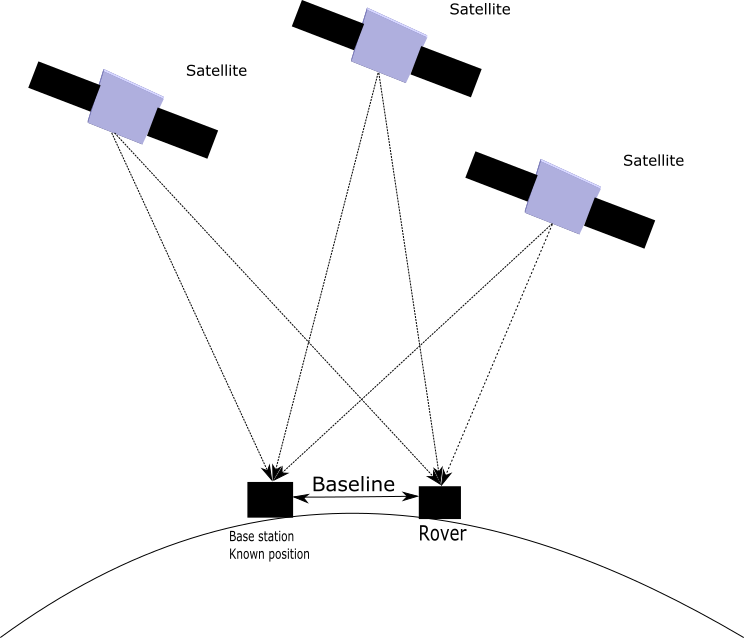
\includegraphics[width=0.7\textwidth]{figs/DGPS.png}
		\caption{Concept figure of \acrfull{dgps}}
		\label{figure:DGPS}
\end{figure}
\section{Error sources}
In order to get high accuracy in the position estimation the different error sources must be identified and removed if possible. This section will identify some of the most significant error sources that can affect the \gls{gnss} signal, and how to remove or mitigate them in the estimation.
\subsection{Clock error}
There is drift in both the satellite clock and the receiver clock. The atomic clock in the satellites makes the clock drift negligible from the user perspective. The receiver clock tend to drift, and if not taken into account will cause large deviations in the position estimate from the true position. This error is remove by including a fourth satellite in the position computation. The satellite clock error is given in the satellite message. 

\subsection{Ionospheric and tropospheric delays}\label{Ss:Atmosphere}
When the \gls{gps} signals travel though the atmosphere there will be a delay caused by the different atmospheric layers.
\subsubsection{Ionospheric delay}
Gas molecules in the ionosphere becomes ionized by the ultraviolet rays that is emitted by the sun, which release free electrons. These electron can influence electromagnetic wave propagation, such as \gls{gnss} signals. In \citep{vik2014integrated} section 3.5.1 it's stated that the delay caused by the ionosphere usually is in the order of $1-10 $meters. The error can be mitigated by using a double frequency receiver, or by applying a mathematical model to estimate the delay. Both those methods are with a single receiver, however by including a second receiver the \gls{gnss} solution system can assume that both receiver receive signal in the same epoch, which means that the signals have experienced the same delay.

\subsubsection{Tropospheric delay}
The tropospheric delay is a function of the local temperature, pressure and relative humidity. From \citep{vik2014integrated} section 3.5.1 the delay can vary from $2.4$ meters to $25$ meters depending on the elevation angle of the satellites. The error can be mitigated by applying a mathematical model to estimate the tropospheric delay, or by using a elevation mask can remove all satellites with a elevation angle bellow a certain threshold. Error caused by tropospheric delay can be removed in the same manners as ionospheric delay when using two or more receivers. 
\subsection{Ephemeris errors}
A satellite is not able to perfectly follow a given orbit, therefore there will be a deviation between satellite position given to the receiver and the true position of the satellite. This is called the ephemeris error. The true position of a satellite is monitored and corrected by the owner of the \gls{gnss} constellation, but error between each correction can be expected.
\subsection{Multipath}
One of the primary source of error in in a GNSS receiver is multipath. Multipath happens when the satellite signal is reflected by a nearby surface before if reach the \gls{gnss} antenna. The delay introduced in the signal can make the receiver believe that its position is several meters away form its true position. The easiest way to mitigated multipath is to place the antenna at a location with open skies, and no tall structures nearby.

Multipath error uncorrelated between receivers, thus the local receiver must be able to correct for multipath error locally.
\cleardoublepage